
\documentclass{standalone}
\usepackage{tikz}
\usetikzlibrary{arrows}

\begin{document}

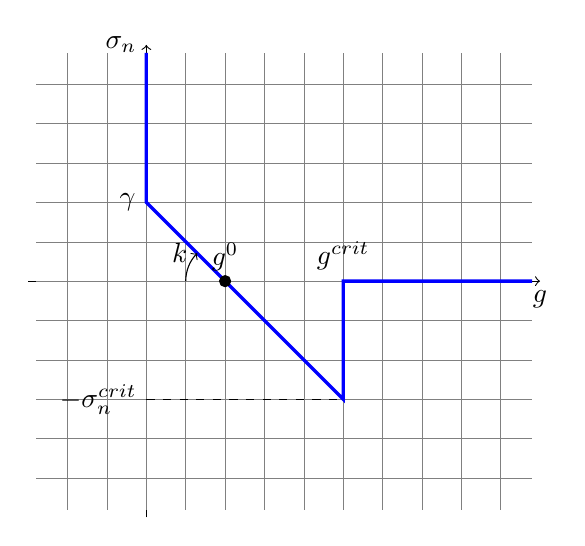
\begin{tikzpicture}
  \draw[->] (-1.5,0) -- (5.,0) node[below]{$g$};
  \draw[->] (0,-3.) -- (0,3.) node[left]{$\sigma_n$};
  \draw[step=0.5cm,gray,very thin] (-1.4,-2.9) grid (4.9,2.9);
  \draw[blue, very thick] (0,2.9) -- (0,1) coordinate (A) node[left,color=black]{$\gamma$} --
                          (2.5,-1.5) coordinate (B) -- (2.5,0) node[above,color=black]{$g^{crit}$} --
                          (4.9,0);
  \draw[dashed] (0,-1.5) node[left]{$-\sigma_{n}^{crit}$} -- (2.5,-1.5);
  \draw[->]  (intersection of -1.5,0--5,0 and A--B) + (-0.5,0) arc (0:-45:-0.5) node[left]{$k$} ;
  \draw[fill] (intersection of -1.5,0--5,0 and A--B) circle (2pt) node[above]{$g^0$};
\end{tikzpicture}

\end{document}
